\documentclass[12pt]{article}

\usepackage{amsmath}
\usepackage{graphicx}
\usepackage{epstopdf}

\begin{document}

\section{Introduction}

\section{Method}

The pendulum is set to follow an angular reference given as a sinusoid 
\begin{equation}
\theta^* = A\sin(2\pi f t + \varphi),
\end{equation}
where the tracking is achieved by a PD - controller, giving the closed-loop system
\begin{equation}
\ddot{\theta} + \zeta\omega_0\dot{\theta} + \omega_0^2\theta = \frac{K_m}{I_f}\left[K_p(\theta^*-\theta) + K_d(\dot{\theta}^*-\dot{\theta})\right]
\end{equation}
where
\begin{equation}
\omega_0 = \sqrt{\frac{m_fgl_f}{I_f}}
\end{equation}
is the undamped resonance frequency, $\zeta$ is a friction term and $K_m$ is the assumed constant gain of the motor. Rearranging the equation gives
\begin{equation}
\ddot{\theta} + \left(\zeta\omega_0 + \frac{K_mK_d}{I_f}\right)\dot{\theta} + \left(\frac{m_fgl_f+K_mK_p}{I_f}\right)\theta = \frac{K_m}{I_f}\left[K_p\theta^*+ K_d\dot{\theta}^*\right]
\end{equation}
where the resonance frequency is now a function of the proportional control term $K_p$ and motor gain $K_m$
\begin{equation}
\omega_{K_P}^2 = \left(\omega_0^2 + \frac{K_mK_p}{I_f}\right) = \left(\frac{m_fgl_f+K_mK_p}{I_f}\right)
\end{equation}
The physical parameters of the pendulum can be further manipulated by attaching weights to each of the legs at fixed known distances from the center of rotation. These weights contributes at torque and moment of inertia according to their attachment point. 
\begin{equation}
\begin{split}
I_w = J_w + (m_w + m_f)(l_s + l_h/2 + (n_w-1)l_h)^2 \\
\tau_w = (m_w + m_f)g(l_s + l_h/2 + (n_w-1)l_h)
\end{split}
\end{equation}
where $n_w \in [0,8]$ is the mounting hole, $l_s$ is the distance to the first mounting hole, $l_h$ is the distance between mounting holes, $m_w$ and $m_f$ is the mass of the weights and fixtures, and $J_w$ is the moment of inertia around the weights center of gravity. The resonance frequency can then be adjusted as 

\begin{equation}
\omega_{K_P}^2  = \left(\frac{m_fgl_f+\tau_w+K_mK_p}{I_f + I_w}\right)
\label{eq:w0kp}
\end{equation}
where $I_w=\tau_w = 0$ if $n_w = 0$. 

Multiple experiments where then carried out with different $K_p$ and $n_w$, and each experiment was ran 3 times to increase statistical significance
\begin{table}
\caption{Table of experiments}
\label{tab:exp}
\begin{center}
\begin{tabular}{c|c|c|c|c|c|c|c|c}
$n_w$ / $K_p$ & 6 & 7 & 8 & 9 & 10 & 11 & 12 & 15 \\ \hline 
(0,0) &   & x & x & x & x & x & x & x\\
(1,1) &   &   & x &   &   &   &   &  \\
(8,8) &   &   & x & x & x &   &   &  \\
(5,5) &   &   & x & x & x &   &   &  \\
(2,8) &   &   & x & x & x &   &   &  \\
(3,7) & x &   & x & x & x &   & x &  \\
(1,0) &   &   & x &   &   &   &   &  \\
(4,0) &   &   & x &   &   &   &   &  \\
(7,0) &   &   & x &   &   &   &   &  
\end{tabular}
\end{center}
\end{table}
The experiments that were performed with $\geq 3$ different $K_p$ values were used to estimate the motor gain $K_m$ by treating $\omega_{K_p}^2$ as a linear function
\begin{equation}
\begin{split}
\omega_{K_P}^2  &= \left(\frac{m_fgl_f+\tau_w+K_mK_p}{I_f + I_w}\right)\\
 y &= ax + b \\
 a = \frac{K_m}{I_f+I_w}, \quad x = K_p, \quad y &= \omega_{K_P}^2, \quad b = \left(\frac{m_fgl_f+\tau_w}{I_f + I_w}\right)
\end{split}
\end{equation}
After obtaining the lumped expression for $\frac{K_m}{I_f+I_w}$, the remaining parameters $m_fgl_f$ and $I_f$ could be found by rearranging \eqref{eq:w0kp} as
\begin{equation}
\begin{split}
\omega_{K_P}^2  &= \left(\frac{m_fgl_f+\tau_w}{I_f + I_w} + aK_p\right)\\
\begin{bmatrix}
1 & -\omega_{K_P}^2 + aK_p 
\end{bmatrix}
\begin{bmatrix}
m_fgl_f \\
I_f
\end{bmatrix}
&=
\omega_{K_P}^2I_w-\tau_w-aK_pI_w 
\end{split}
\end{equation}
for each experiment in Table \ref{tab:exp}, and constructing an overdetermined set of equations on the form
\begin{equation}
Ax=b
\end{equation}
where $ x = [m_fgl_f, I_f]^T$, and the solution is given by least-squares fitting as
\begin{equation}
x = \left(A^TA\right)^{-1}b.
\end{equation}

\section{Results}

\begin{figure}[htbp]
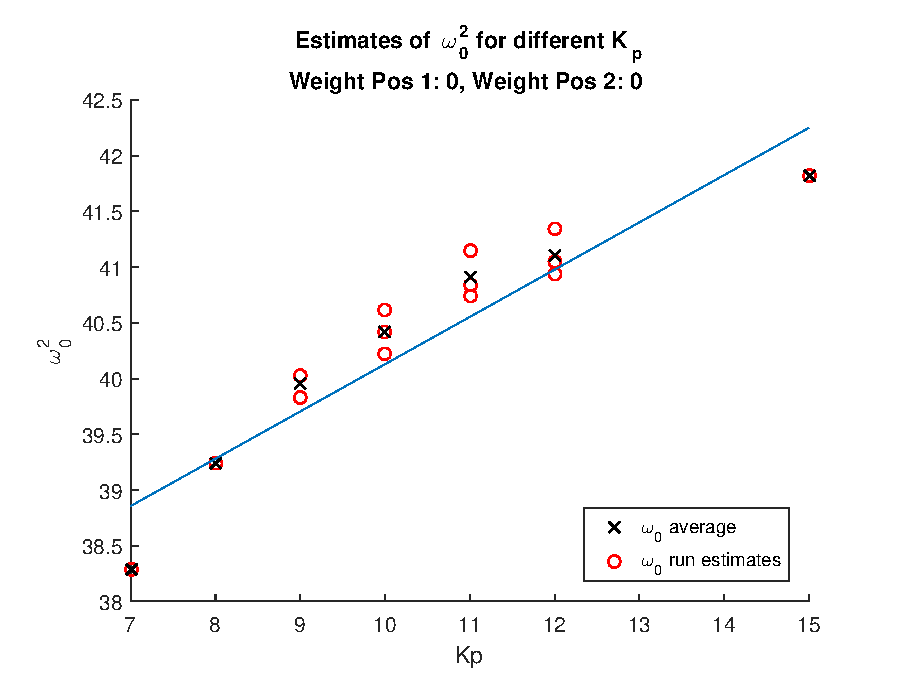
\includegraphics[scale=1]{gfx/km_00}
\label{fig:km_00}
\caption{Estimated linear fit for $\frac{K_m}{I_f+I_w}$ parameter for experiments without weights attached.}
\end{figure}

\begin{figure}[htbp]
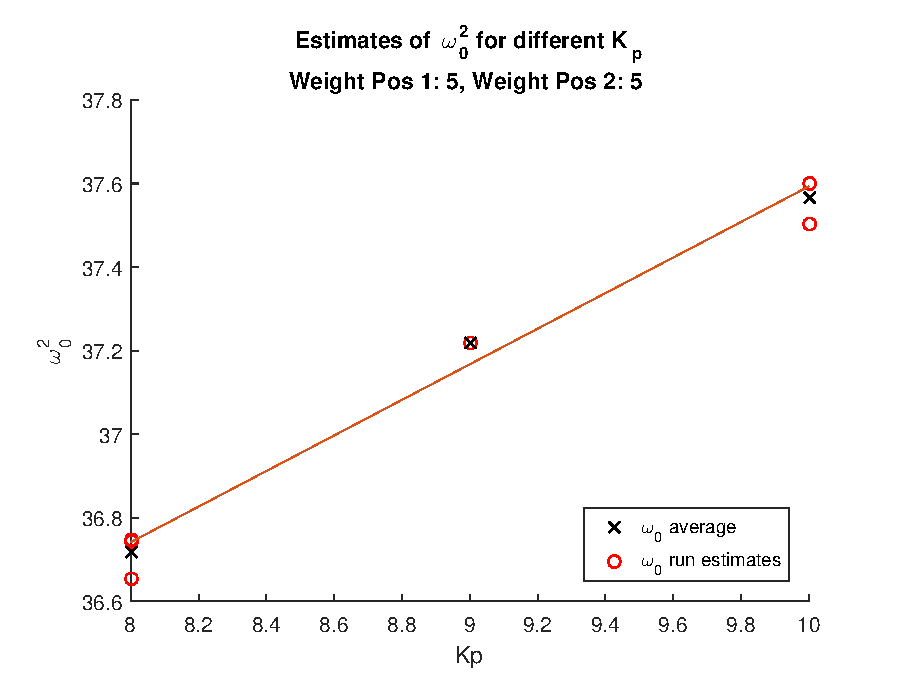
\includegraphics[scale=1]{gfx/km_55}
\label{fig:km_55}
\caption{Estimated linear fit for $\frac{K_m}{I_f+I_w}$ parameter for experiments with weights attached at $n_w = (5,5)$.}
\end{figure}

\begin{figure}[htbp]
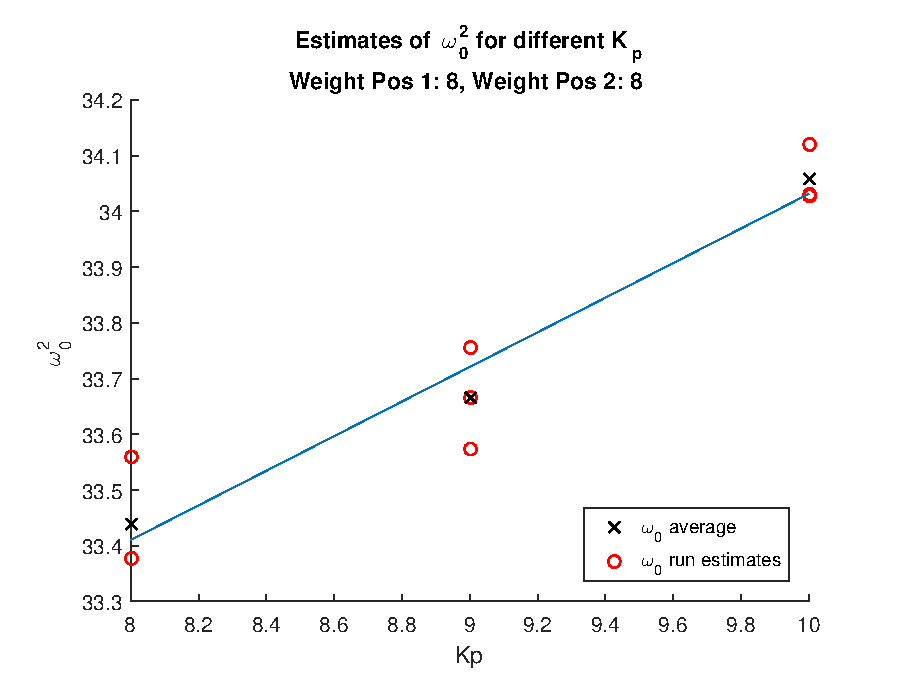
\includegraphics[scale=1]{gfx/km_88}
\label{fig:km_88}
\caption{Estimated linear fit for $\frac{K_m}{I_f+I_w}$ parameter for experiments with weights attached at $n_w = (8,8)$.}
\end{figure}

\begin{figure}[htbp]
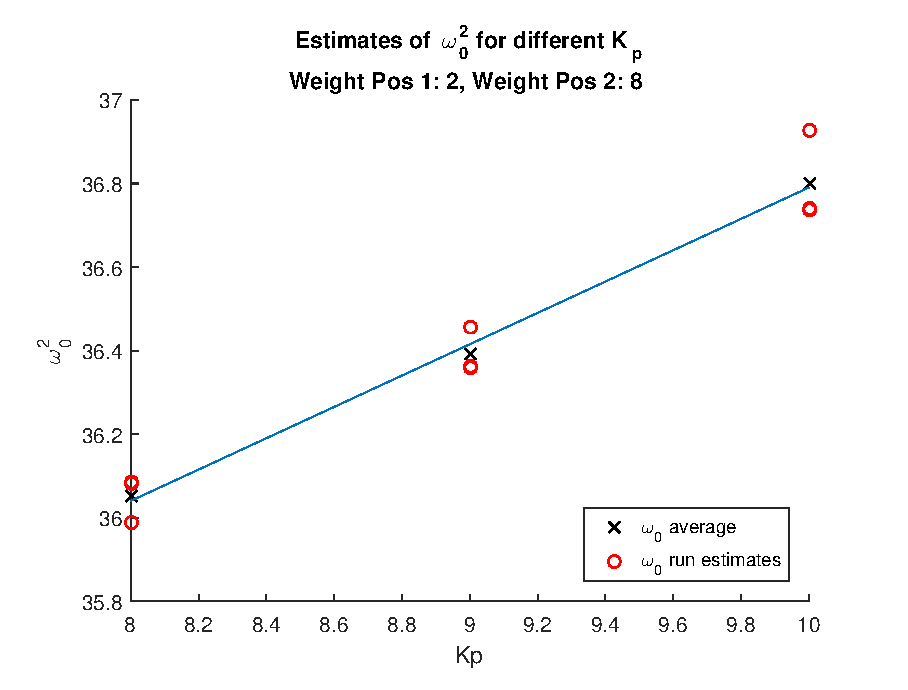
\includegraphics[scale=1]{gfx/km_28}
\label{fig:km_28}
\caption{Estimated linear fit for $\frac{K_m}{I_f+I_w}$ parameter for experiments with weights attached at $n_w = (2,8)$.}
\end{figure}

\begin{figure}[htbp]
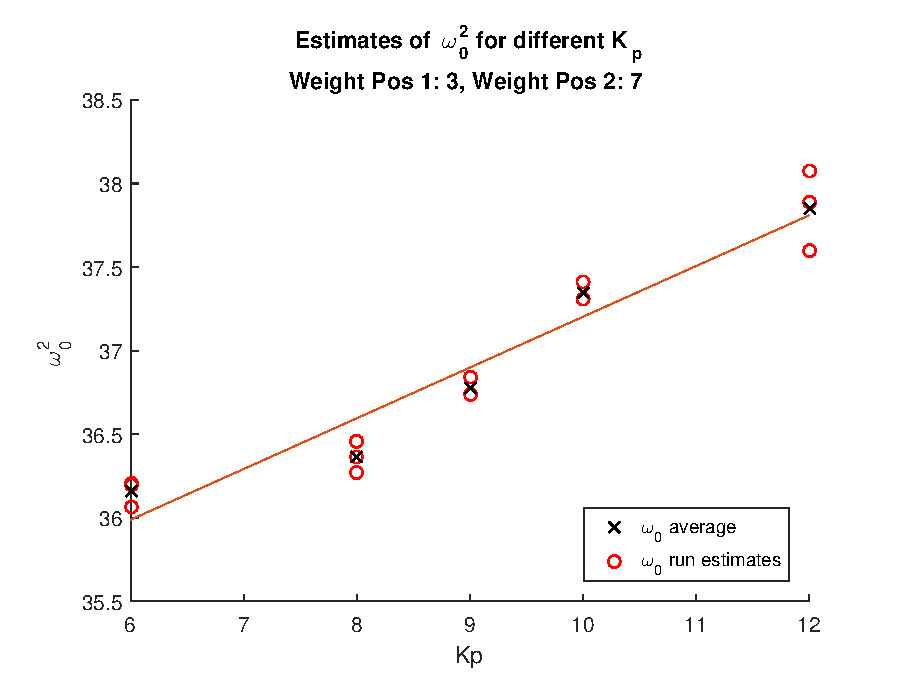
\includegraphics[scale=1]{gfx/km_37}
\label{fig:km_37}
\caption{Estimated linear fit for $\frac{K_m}{I_f+I_w}$ parameter for experiments with weights attached at $n_w = (3,7)$.}
\end{figure}

\begin{table}
\caption{Motor gain estimates}
\label{tab:km}
\begin{center}
\begin{tabular}{c|c}
$n_w$ & $\frac{K_m}{I_f+I_w}$ \\ \hline 
(0,0) &   0.424071985869166\\
(8,8) &  0.310548831022341 	\\
(5,5) & 0.425654308341756 \\
(2,8) & 0.374895472210993 \\
(3,7) & 0.303311751403483 \\
\end{tabular}
\end{center}
\end{table}

\begin{table}
\caption{Parameter estimates}
\label{tab:param}
\begin{center}
\begin{tabular}{c|c}
$m_fgl_f$  & 7.213988198586391\\
$I_f$ & 0.200275108832547\\
$K_m$ & 0.096860674406427\\
\end{tabular}
\end{center}
\end{table}

\begin{table}
\caption{Verification experiments}
\label{tab:km}
\begin{center}
\begin{tabular}{c|c|c|c}
$n_w$ & $\omega_0^*$ & $\omega_0$ & error \\ \hline 
(1,1) &      6.341697809300672 &   6.375158252674985 &  -0.033460443374313 \\
(1,0) &     6.297273096333526 	&   6.347945772068390 &  -0.050672675734864	\\
(4,0) &    6.182221951346674 &   6.221128813138584 &  -0.038906861791911\\
(7,0) &    6.022659862653705&   6.037844301505593 &	  -0.015184438851888
\end{tabular}
\end{center}
\end{table}


\section{Conclusion}

\end{document}